\documentclass[9pt]{beamer}

%-------------------------------------------------
%   THEMES & PACKAGES
%-------------------------------------------------
\usetheme[progressbar=frametitle]{metropolis}
\usepackage{graphicx}
\usepackage[export]{adjustbox}

%-------------------------------------------------
%   TITLE
%-------------------------------------------------
\title{Advanced Mathematics for Robotics and Control}
\subtitle{Bishop Book Chapter 1}
\date{Lecture date: October 6, 2016}
\author{Minh Nguyen}
\titlegraphic{\hfill
\includegraphics[height=0.7cm]{../../images/h-brs-logo.jpg}}

%-------------------------------------------------
%   BEGIN
%-------------------------------------------------
\begin{document}

%-------------------------------------------------
\maketitle

%-------------------------------------------------
%-------------------------------------------------
\begin{frame}{Review}
    \begin{alertblock}{General terms}
        Training set, test set, learning phase, input vector, target vector, feature extraction, ...
    \end{alertblock}
    \begin{alertblock}{Result of machine learning algorithm}
        Produces function $y(x)$ which can take new input and generates an output vector $y$ encoded in the same way as target vectors.
    \end{alertblock}
    \begin{alertblock}{Generalisation}
        Ability to categorize correctly new examples.
    \end{alertblock}
    \begin{alertblock}{Learning approaches}
        \textbf{Supervised:} input and target vectors are known, can be either regression (continuous variables) or classification (finite discrete categories).\\
        \textbf{Unsupervised:} data only contain inputs, no target is known.\\
        \textbf{Reinforcement learning:} discover output through a number of trial and errors, in order to maximize a reward.
    \end{alertblock}
\end{frame}

%-------------------------------------------------
%-------------------------------------------------
\begin{frame}{Probability Theory}
    \begin{alertblock}{Rules of Probability}
        \textbf{Sum rule:}
        \[ p(X) = \sum_{Y}^{} p(X, Y) \]
        \textbf{Product rule:}
        \[ p(X, Y) = p(Y | X) p(X) \]
        where $p(X, Y)$ is a joint probability, $p(Y | X)$ is a conditional probability, $p(X)$ is a marginal probability.

        \textbf{Bayes' theorem} can be directly obtained from the product rule and the symmetry property $p(X,Y) = p(Y,X)$:
        \[ p(Y | X) = \cfrac{p(X|Y) p(Y)}{p(X)} \]
    \end{alertblock}
\end{frame}

%-------------------------------------------------
%-------------------------------------------------
\begin{frame}{Probability Theory}
    \begin{alertblock}{Prior and posterior}
        \textbf{Example:} probability of selecting the red box is $P(B = r) = 4/10$.
        What is the color of the box if we pick a piece of fruit from the boxes?\\
        Observation: the fruit is orange.
        \begin{center}
            \setlength{\fboxsep}{0.5pt} %
            \setlength{\fboxrule}{0.5pt}
            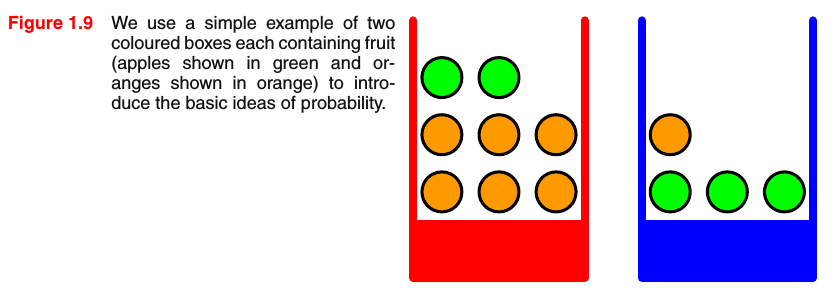
\includegraphics[width=7.0cm,fbox]{../images/Bishop_MachineLearning_Figure1-9.png} %
        \end{center}
        \textbf{Prior probability:} $P(B)$, provided before the identity of the fruit (variable $F$) is observed.\\
        \textbf{Posterior probability:} $P(B|F)$, probability obtained after $F$ is observed.
        \[ p(B=r|F=o) = \cfrac{p(F=o|B=r)p(B=r)}{p(F=o)} = \frac{6}{8} \times \frac{4}{10} \times \frac{20}{9} = \frac{2}{3} \]
    \end{alertblock}
\end{frame}

%-------------------------------------------------
%-------------------------------------------------
\begin{frame}{Probability Theory}
    \begin{alertblock}{Probability densities}
        \begin{center}
            \setlength{\fboxsep}{0.5pt} %
            \setlength{\fboxrule}{0.5pt}
            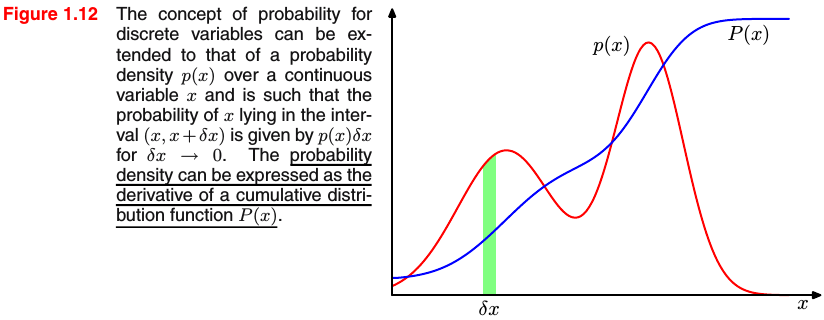
\includegraphics[width=7.0cm,fbox]{../images/Bishop_MachineLearning_Figure1-12.png} %
        \end{center}
        \textbf{Cumulative distribution function:} gives the probability that variable $x$ lies in interval $(-\infty, z)$:
            \[ P(z) = \int_{-\infty}^{z} p(x) dx \]
        \textbf{Requirements on probability density function:}
            \[ p(x) \geq 0, \int p(x) dx = 1 \]
        \textbf{Sum and product rules:} $p(x) = \int p(x, y) dy, p(x, y) = p(y|x) p(x)$
    \end{alertblock}
\end{frame}

%-------------------------------------------------
%-------------------------------------------------
\begin{frame}{Probability Theory}
    \begin{alertblock}{Expectations and covariances}
        \textbf{Expectation of some function $f(x)$:} average value of $f(x)$ under a probability distribution $p(x)$, denoted $\mathbb{E}[f]$:\\
            Discrete: $\mathbb{E}[f] = \sum_x p(x)f(x)$\\
            Continuous: $\mathbb{E}[f] = \int p(x)f(x)dx$\\
        \textbf{Conditional expectation:}
            \[ \mathbb{E}_x[f|y] = \sum_x p(x|y)f(x) \]
            where $\mathbb{E}_x[f(x, y)]$ is average of $f(x,y)$ with respect to the distribution of $x$\\
        \textbf{Variance of $f(x)$:}
            \[ var[f] = \mathbb{E} \left[ (f(x) - \mathbb{E}[f(x)])^2 \right] = \mathbb{E}[f(x)^2] - \mathbb{E}[f(x)]^2 \]
        \textbf{Covariance:} for two random variables $x$ and $y$:
            \[ cov[x,y] = \mathbb{E}_{xy}[xy] - \mathbb{E}[x]\mathbb{E}[y] \]
            if $x$ and $y$ are vectors: $cov[x,y] = \mathbb{E}_{xy}[xy^T] - \mathbb{E}[x]\mathbb{E}[y^T]$
    \end{alertblock}
\end{frame}

%-------------------------------------------------
%-------------------------------------------------
\begin{frame}{Probability Theory}
    \begin{alertblock}{Bayesian Probabilities}
        \begin{itemize}
            \item Probabilities provides quantification of uncertainty
            \item Bayes' theorem can be used to covert a \underline{prior} probability to a \underline{posterior} probability
                by \underline{incorporating evidence} provided by the observed data (i.e. orange apple example)
        \end{itemize}
    \end{alertblock}
    \begin{alertblock}{Likelihood function}
        Consider uncertainty problem with parameters $w$, prior priority $p(w)$ before data $\mathcal{D}$ is observed.\\
        Bayes theorem: $p(w|\mathcal{D}) = \cfrac{p(\mathcal{D}|w) p(w)}{p(\mathcal{D})}$\\
        Conditional probability $p(\mathcal{D}|w)$ can be viewed as a function of $w$ and called a \textbf{likelihood function}.\\
        \textbf{Error function: } negative log of the likelihood function (machine learning).
    \end{alertblock}
\end{frame}

%-------------------------------------------------
%-------------------------------------------------
\begin{frame}{Probability Theory}
    \begin{alertblock}{Gaussian distribution}
        With mean $\mu$ and variance $\sigma^2$:
        \[ \mathcal{N}(x|\mu,\sigma^2) = \cfrac{1}{(2\pi \sigma^2)^{1/2}}exp\left\{-\cfrac{1}{2\sigma^2}(x - \mu)^2\right\} \]
        \begin{center}
            \setlength{\fboxsep}{0.5pt} %
            \setlength{\fboxrule}{0.5pt}
            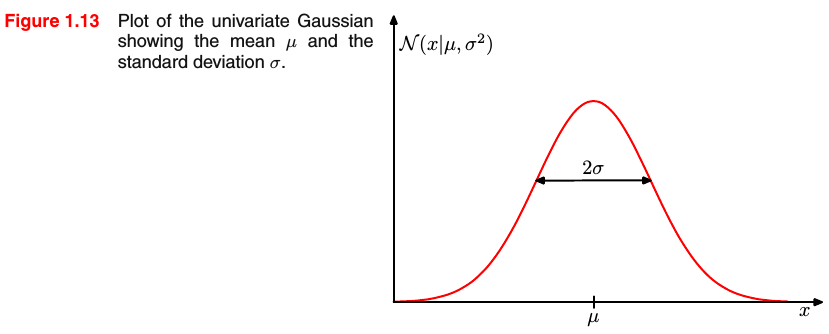
\includegraphics[width=7cm,fbox]{../images/Bishop_MachineLearning_Figure1-13.png} %
        \end{center}
        If data set $\mathbf{x}$ is i.d.d. from a Gaussian distribution with unknown $\mu$ and $\sigma^2$, likelihood function of data set:
        \[ p(\mathbf{X}|\mu, \sigma^2) = \prod_{n=1}^{N}\mathcal{N}(x_n|\mu, \sigma^2) \]
        %Maximizing the log likelihood function can find $\mu_{ML}$ and $\sigma_{ML}^2$
    \end{alertblock}
\end{frame}

%-------------------------------------------------
%-------------------------------------------------
\begin{frame}{Model Selection}
    \begin{alertblock}{Cross Validation}
        \begin{center}
            \setlength{\fboxsep}{0.5pt} %
            \setlength{\fboxrule}{0.5pt}
            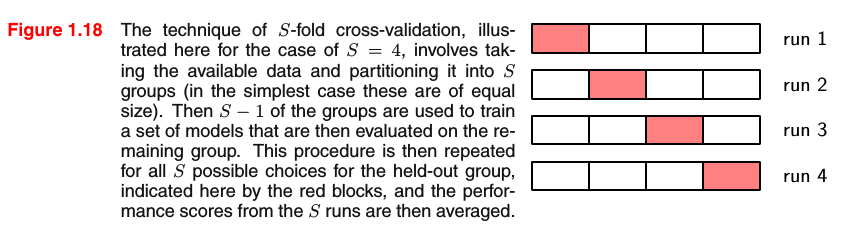
\includegraphics[width=7cm,fbox]{../images/Bishop_MachineLearning_Figure1-18.png} %
        \end{center}
        Drawbacks:
        \begin{itemize}
            \item Number of training runs is increased by a factor of $S$
            \item Models can have multiple complexity parameters $\rightarrow$ number of training runs exponential in number of parameters
        \end{itemize}
    \end{alertblock}
\end{frame}

%-------------------------------------------------
%-------------------------------------------------
\begin{frame}{Curse of Dimensionality}
    Example: oil flow data. 'Homogeneous' class is red, 'annular' is green, and 'laminar' is blue.
    New test point denoted by 'x' is to be classified.
    \begin{center}
        \setlength{\fboxsep}{0.5pt} %
        \setlength{\fboxrule}{0.5pt}
        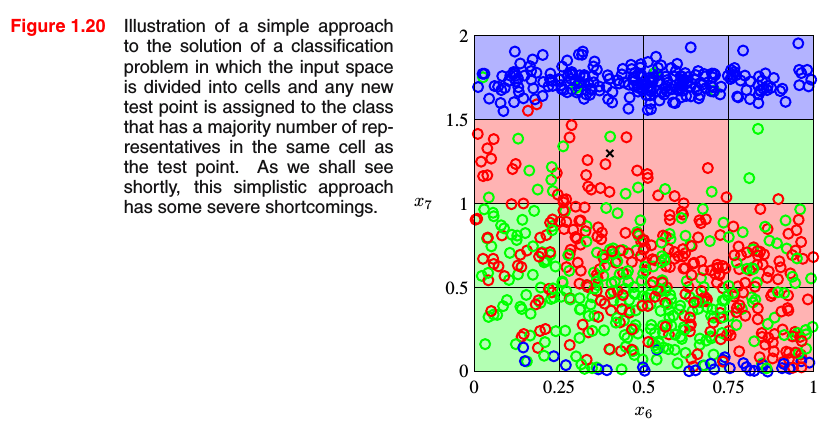
\includegraphics[width=7cm,fbox]{../images/Bishop_MachineLearning_Figure1-20.png} %
    \end{center}
    Example: Polynomial curve fitting with $D$ input variables. Polynomial with coefficients up to order 3:
    \begin{center}
        \setlength{\fboxsep}{0.5pt} %
        \setlength{\fboxrule}{0.5pt}
        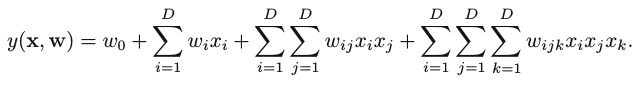
\includegraphics[width=7cm,fbox]{../images/Bishop_MachineLearning_Eq1-74.png} %
    \end{center}
\end{frame}

%-------------------------------------------------
%-------------------------------------------------
\begin{frame}{Decision Theory}
    \begin{alertblock}{Minimizing the classification rate}
        \begin{center}
            \setlength{\fboxsep}{0.5pt} %
            \setlength{\fboxrule}{0.5pt}
            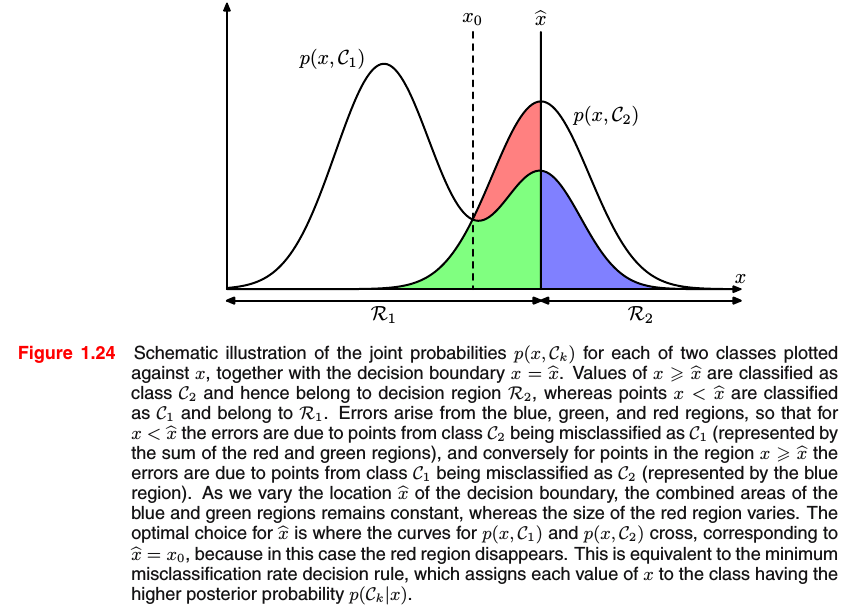
\includegraphics[width=10cm,fbox]{../images/Bishop_MachineLearning_Figure1-24.png} %
        \end{center}
    \end{alertblock}
\end{frame}

%-------------------------------------------------
%   END
%-------------------------------------------------
\end{document}
